


\chapter{L'aspect bloquant du réseau}
Dans ce chapitre, les principales problématiques data centre sous un aspect réseau seront présentées et analysées. Seront abordés quelques questionnements sur les réseaux classiques pour tenter de répondre aux nouveaux besoins data centres. Le chapitre présentera comment divers scénarios sont traités aujourd'hui et quelles en sont les limites. 


\section{Le rôle du réseau dans les projets de TI}

Lors du développement de projets pour l'optimisation en \gls{ti} telles que la consolidation de data centres et la virtualisation de serveurs, une attention spéciale doit être donnée au rôle critique des réseaux dans la planification, l'exécution et succès en général du projet. Il est souvent admis que des planifications supplémentaires par rapport aux réseaux auraient pu contribuer au succès de plusieurs projets.

%As organizations undertake information technology (IT) optimization projects, such as data center consolidation and server virtualization, they need to ensure that the proper level of focus is given to the critical role of the network in terms of planning, execution, and overall project success. While many consider the network early in the planning stages of these projects and spend time considering this aspect of these initiatives, many more feel that additional network planning could have helped their projects be more successful.


Les principaux types de modifications dans ces projets incluent l'implémentation d'équipement réseau supplémentaire pour augmenter ou améliorer la redondance, la capacité du réseau, la sécurité réseau et/ou la bande passante. Cependant, plusieurs requis associés à ces changements ne sont pas, en général, identifiés au tout début du projet. Très souvent ils ne sont détectés qu'après les étapes initiales du projet, imposant un supplément de travail et l'ajout de coûts non anticipés.

%The most common types of network changes in IT optimization projects include implementing new network equipment, adding greater redundancy, increasing capacity by upgrading switches, improving network security, and adding network bandwidth. However, many network requirements associated with these changes and the overall initiative are typically not identified until after the initial stages of the project and often require rework and add unanticipated costs. Regardless of project type, network challenges run the risk of contributing to increased project time lines and/or costs.


Les aspects réseau d'un projet peuvent être difficiles à gérer, et des critiques sur le fonctionnement général des réseaux sont fréquemment entendues. Des défis importants incluent la réalisation d'analyses des causes précises et opportunes, la compréhension de la réactivité au niveau applicatif et la révélation des origines de problèmes de performance. Le simple achat d'équipement réseau n'aborde pas nécessairement ou proprement les requis réels.

%The networking aspects of projects can be challenging and user complaints about the network are frequently heard. Important challenges include the inability to perform accurate and timely root-cause analysis, understand application level responsiveness, and address network performance issues. Simply buying more network equipment does not necessarily or appropriately address the real requirements.


%Looking ahead, many expect that the network will become more important to their companies' overall success. To address this, networking investments related to support of server and storage virtualization are currently at the top of the list for consideration, followed by overall enhancement and optimization of the networking environment. To support virtualization of the entire IT infrastructure and to continue to optimize the network, IT organizations need to make architectural decisions in the context of the existing infrastructure, IT strategy, and overall business goals.


Pour supporter la virtualisation complète d'une infrastructure de \gls{ti} et continuer à optimiser le réseau, des décisions sur l'architecture doivent être faites dans le contexte de l'infrastructure existante, de la stratégie et des objectifs larges du business. Sans le développement d'un plan réseau et la conception fonctionnelle associée, les transitions réseau peuvent être risquées et conduire à un contrôle réduit des services livrés, coûts potentiellement élevés contre des résultats insuffisants et des problèmes inattendus de performance ou disponibilité. 
%Developing a plan for the network and associated functional design is critical. Without a strong plan and a solid functional design, networking transitions can be risky, leading to reduced control of IT services delivered over the network, the potential for high costs with insufficient results, and unexpected performance or availability issues for critical business processes.

%The network is the natural home for management and enforcement of policies relating to risk, performance, and cost. Only the network sees all data, connected resources, and user interactions within and between clouds. The network is thus uniquely positioned to monitor and meter usage and performance of distributed services and infrastructure. Management tools for the data center and wider networks have moved from a user-centric focus (for example, GUI design) to today’s process-centric programmatic capabilities. In the future, the focus will most likely shift toward behavioral- and then cognitive-based capabilities.
%The network also has a pivotal role to play in promoting resilience and reliability. For example, the network, with its unique end-to-end visibility, helps support dynamic orchestration and redirection of workloads through embedded policy-based control capabilities. The network is inherently aware of the physical location of resources and users. Context-aware services can anticipate the needs of users and deploy resources appropriately, balancing end-user experience, risk management, and the cost of service.

Traditionnellement un plan et une conception fonctionnelle solides suffisaient pour augmenter le succès des projets avec un réseau réactif, optimisé, moins cher et répondant mieux aux engagements des services applicatifs. Alors que ce plan reste essentiel, il est difficile dans le contexte d'utilisation actuel de maitriser complètement  à l'avance la charge, dimension et tout autre requis qui doivent être assurés par les réseaux.

Face à ces difficultés et aux critiques reçues, il est facile d'en venir à considérer les réseaux comme un élément bloquant pour le succès des projets. Même si la gestion et la planification peuvent être complexes, les réseaux représentent un moyen naturel pour manager et renforcer les politiques liées aux risques, performance et coûts. Cependant, le réseau voit toutes les données, ressources connectées et interactions des utilisateurs à travers le Cloud. Le réseau est donc positionné de manière unique pour surveiller et mesurer l'usage et la performance des services distribués et de l'infrastructure. Les réseaux ont également un rôle central pour favoriser l'extensibilité et disponibilité. Par exemple avec leur vue unique bout-en-bout, les réseaux peuvent détecter la charge et dynamiquement la rediriger selon les politiques de contrôle.

Afin d'atteindre ce niveau de management et orchestration des ressources, on cherche  à concevoir des architectures réseaux qui puissent s'étendre ou se rétracter ainsi que supporter des nouveaux services de façon dynamique et rapide en fonction des besoins immédiats. \cite{ibmPlanningVirtCCchap4} \cite{cloudAutomation} \cite{hpCloudEffectsOnNetworkIntro}
%With a plan and a solid functional design, the probability of success is raised: a more responsive network with optimized delivery, lower costs, increased ability to meet application service level commitments, and a network that supports and fully contributes to a responsive IT environment.


\section{L'architecture réseau d'un data centre typique}

La majorité des data centres d'aujourd'hui ont une structure réseau hiérarchique à trois niveaux : couche d'accès, agrégation/distribution et cœur (figure \ref{legacy_archi}). La couche d'accès inter-connecte toutes les ressources partagées telles que serveurs, dispositifs de stockage et applications. Les réseaux d'agrégation (ou distribution) doivent fournir une haute bande passante pour la communication entre multiples réseaux d'accès. Le cœur du réseau est l'interface vers l'extérieur du réseau, qui peut être le lien avec des réseaux WAN, mobiles, VPNs ou autres types d'accès internet. \\
%The access network provides connectivity to all shared enterprise servers, applications, storage devices, and any IP or office automation devices required in the data center facility. Most data center access switches are deployed at the top of the rack or at the end of the row of server racks.

%Most data centers today have a three- or four-tier hierarchical networking structure. It consists of access layer switches, aggregation switches, and core switches (Figure 1). Three-tier networking architectures were designed around client-server applications and single-purpose application servers. Client-server applications caused traffic to flow primarily in North/South (N/S) patterns: from a server up to the data center core, to the campus core where it moves out to the campus-wide network or internet. These large core switches usually contain the vast majority of the intelligence in the network.


\begin{figure}[h]
\begin{center}
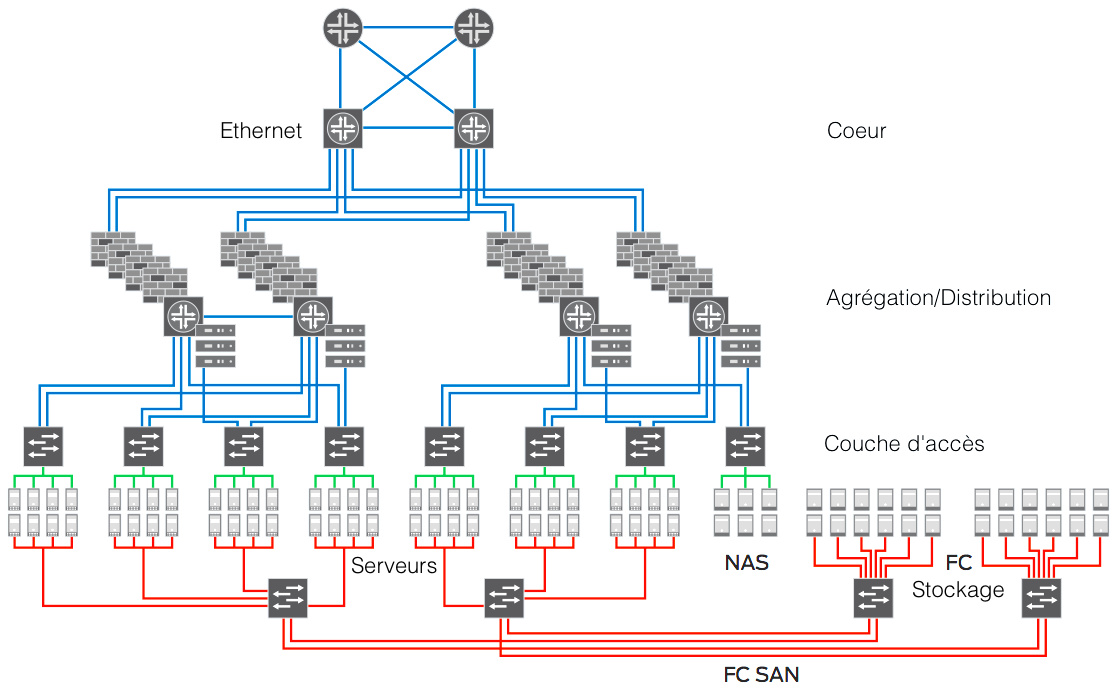
\includegraphics[width=0.8\textwidth]{images/LegacyNetworkArchitecture} 
\caption{Architecture réseau typique à trois niveaux. \cite{cloudReadyNetworkJuniper}} \label{legacy_archi}
\end{center}
\end{figure}



%The core network provides a fabric for high-speed packet switching between multiple access network devices. Due to their location in the network, core-layer switches must provide scalable, high-performance, high-density, wire-rate ports, and HA hardware and software features that deliver carrier-class reliability and robustness. The core serves as the gateway where all other modules such as the WAN edge meet. It typically requires a 10GbE interface for high-level throughput, and maximum performance to meet oversubscription levels. The core provides high-speed throughput for all data going into and out of the data center, and it must provide resilient, fail-safe Layer 3 connectivity to multiple access layer devices.


%The edge network provides the communication links to end user networks of various types. These can be private WAN or campus backbones, mobile access networks, VPNs, or other types of Internet access. The high performance and reliability of these connections improve user experience. Agility ensures that users will have access to applications and services where and when they are needed. In addition, multilayered security controls ensure that users, applications and data are protected at appropriate levels.

Cette architecture a été conçue pour les applications client-serveurs dans des serveurs applicatifs dédiés. Dans cette conception, le flux du trafic se fait essentiellement à partir des serveurs en direction du cœur du réseau et ensuite en dehors vers internet ou autre (flux Nord/Sud).

Ce modèle d'architecture a été la principale référence de topologie réseau pour les data centres. Cependant, il devient complexe à le maintenir dans le contexte du Cloud Computing lorsque les applications actuelles commencent à être plus distribuées, avec plusieurs couches et orientées livraison de services. Ces changements dans les applications ont impacté les réseaux pour ce qui concerne le volume et les flux du trafic. 

Le trafic réseau interne a augmenté avec la croissance du nombre d'applications et services déployés ; l'utilisation de systèmes de fichiers distribués avec des données stockées séparément a eu pour conséquence une charge réseau plus importante à travers le data centre. De ce fait, on constate une forte tendance de communications inter-serveurs ou inter-VMs, impliquant un flux Est/Oust plutôt que Nord/Sud. L'industrie estime même que 80\% du trafic des applications Cloud Computing constitue des flux Est/Ouest.

%Industry sources attribute up to 80 percent of network traffic for these next generation applications coming from E/W traffic flows.

%This network architecture, however, is becoming problematic for the data center. Today’s application environments are more distributed, often with multiple tiers, and oriented toward service delivery. These application architecture changes have resulted in:
%• Greater traffic volume on the Ethernet network, including storage traffic such as FCoE and iSCSI
%• More storage traffic as applications use distributed file systems and increase the amount of synchronization and replication data across the network
%• Greater traffic flow between peer servers such as server-to-server or virtual machine-to-virtual machine—that is, East/West (E/W) rather than primarily N/S traffic flows.

Cette architecture révèle une série d'interfaces de connexions des serveurs à divers types de réseaux tels que réseaux locaux, de stockage, communication entre processus. Cette disposition ajoute de la complexité et des coûts sous forme de câblage, nombre de ports, extensibilité, énergie, refroidissement etc. 

Les data centres d'aujourd'hui exigent des réseaux agiles et flexibles pour pouvoir réagir rapidement aux changements et garantir une livraison efficace de services. Par exemple, des serveurs virtuels peuvent être déplacés de part et d'autre avec une simple commande en fonction de la demande. Par conséquent, les réseaux doivent s'adapter rapidement à ces changements pour éviter des perturbations du service. Cela suppose que les dispositifs apparaissent connectés au même réseau local, indépendamment de leur proximité physique. Il manque à cette architecture la flexibilité nécessaire pour effectuer ces types de changements, ce qui impacte défavorablement l'efficacité opérationnelle de tout le data centre.
%today’s data center, demands networks that are nimble and adaptable enough to react quickly to changes and maintain efficient delivery of mission critical services. Virtual servers, for example, can be moved from one part of the data center to another with a simple command to better meet demand, and networks must adapt quickly to these changes or risk service disruption. Such changes require that devices appear to be seamlessly connected on the same laN, regardless of their physical proximity to each other. legacy network architectures lack the flexibility to react to these types of changes, and this adversely affects the operational efficiency of the entire data center.
%In addition to the way boxes are physically connected and oriented, keeping the network running becomes a challenge  when existing technologies prevent network engineers from doing their jobs efficiently. everyday tasks such as monitoring devices, troubleshooting, configuration management, and software upgrades become increasingly difficult as the number of independent devices in the network increases.
%Such operational challenges are further compounded if these devices are running different versions of software or have different configurations, since software must be carefully managed across devices to ensure consistent functionality and limit exposure to bugs or other vulnerabilities. Special training or expertise may also be needed to support these configurations. as a result, the manpower required to adequately operate, maintain, and troubleshoot the unique requirements of each network device can be enormously time-consuming and costly.


Afin de mieux visualiser ces difficultés, quelques scénarios critiques pour les réseaux traditionnels seront étudiés en détail. Ces scénarios supposent des infrastructures basées sur cette architecture à trois niveaux (présentée précédemment) et avec l'objectif de fonctionner en mode Cloud Computing.  \cite{cloudReadyNetworkJuniper} \cite{hpCloudEffectsOnNetworkChanging} \cite{cloudReadyJuniperReferenceNetworkInfra} \cite{bigDataBookChap4}

\section{La transformation des applications et exemples de scénarios critiques}

Avec de multiples VMs s'exécutant chez le même hôte, partageant une carte réseau unique au moyen d'un switch logiciel (ou virtuel), les applications ont donc moins de ressources réseau que lorsqu'un serveur physique leur est dédié. Cela peut conduire à des problèmes de performance réseau comme une bande passante réduite et un temps de latence augmenté et même à d'autres difficultés mineures comme la disponibilité de plages d'adresses IP ; les applications peuvent ne pas être en mesure de traiter ces questions.


%With a physical machine running a network application, that application can have access to the full resources of the network card. Once 10 virtual machines are running together on a single host—sharing a single hardware network card and streaming together through a software switch—that same virtualized application now has fewer networking resources available than it did before. This can lead to overall network performance issues, reduced bandwidth, and increased latency; all issues the application might not be able to deal with. Even smaller issues such as IP address availability can be impacted by virtualization sprawl.


Les plateformes typiques d'infrastructure virtuelle fournissent des logiciels pour faire migrer les instances de VMs actives d'un dispositif physique à l'autre; VMware Distributed Resource Scheduler (DRS) et VMotion sont des exemples de ce type de solutions. Ces solutions ne connaissent pas l'état des applications ou du réseau. Par exemple, une VM peut être migrée au milieu d'une transaction bancaire sans prendre en compte l'état de persistance de l'opération, le nombre des connexions ou la charge réseau que la VM est en train de traiter. Cela peut causer des transactions non réussies, avec perte de données et problèmes plus graves pour les utilisateurs. Par ailleurs, ces technologies permettent de migrer une VM vers un serveur physique avec plus de charge CPU disponible, mais elles n'ont pas d'informations sur la capacité réseau dans ce serveur.  
%Virtual infrastructure platforms typically include software that can migrate live virtual machine instances from one physical device to another; VMware Distributed Resource Scheduler (DRS) and VMotion are examples of live migration solutions. Like basic OS virtualization, these migration tools are unaware of the application state, and also have no insight into the Application Delivery Network. For example, VMotion may move a virtual machine running a web shopping cart application from one host server to another without taking into consideration the current persistent state of user’s carts, how many connections are coming into the shopping cart, or the network load that this particular virtual machine is currently handling. This migration can cause a lapse in availability; connections to the application and application persistence for the user can be lost during this live migration, resulting in failed transactions, lost shopping cart data, and frustrated users. And while VMotion attempts to move the live image to a host server that is under less load, VMotion doesn’t measure the network load of that host device. It might move a live image to a machine with more available CPU cycles but less available network capacity.



Le déplacement dynamique de charges exige également que les VMs restent dans un VLAN commun, dans le même réseau au niveau 2.  Pour pouvoir déplacer un réseau en dehors de son domaine niveau 2, il est nécessaire d'utiliser des procédures manuelles comme l'attribution d'adresses IP et mise à jour des entrées DNS pour les services déplacés. Pour maximiser cette flexibilité, des technologies émergent pour élargir le domaine des réseaux au niveau 2.

%Moving workloads dynamically requires VMs to stay within a common VLAN in the same Layer 2 (L2) network. If you want to move a VM outside its L2 domain, you have to use manual processes such as assigning and updating the IP addresses for the failed-over services and updating DNS entries correctly. To provide maximum VM flexibility, many enterprises are evaluating ways to enlarge their L2 networks.

De nouveaux moyens tels que  \gls{vxlan} et \gls{nvgre} étendent les réseaux couche 2 avec des réseaux couche 3. Même si cette capacité devient possible avec ces technologies, le trafic local aura toujours une meilleure performance et une latence inférieure s'ils restent dans un réseau niveau 2. 
\cite{hpCloudEffectsOnNetworkChanging} \cite{vm7Challenges} \cite{zkCloudArrived}


%Parce que le rôle des réseaux a changé, les stratégies classiques ne suffisent plus pour 
%Because the role of the network has changed, current network strategies are no longer sufficient to enable a shift to the cloud. The network has shifted from a tactical, best-effort resource to a key enabler, raising corporate productivity to unprecedented levels. Customers that do not embrace the network as a foundation for cloud delivery put their organizations at risk, as users will experience inconsistent application performance, security exposure and poor business continuity. Leveraged correctly, the network plays a key role helping any organization shift business applications to the cloud.



%New capabilities such as Virtual eXtensible LAN (VXLAN) and Network Virtualization using Generic Routing Encapsulation (NVGRE) logically extend an L2 network across L3 networks. However, even with this potential to move VMs across a L3 network, local traffic will still have higher performance and lower latency if it stays within a large L2 network.

\subsection{Aspect multi-tenant}

Cet exemple traite l'aspect multi-tenant des infrastructures Cloud. Pour simplifier, on considère une configuration avec deux réseaux : un pour le groupe d'ingénieurs et l'autre pour l'équipe des ventes. Pour réaliser cela avec les technologies réseaux traditionnelles, on utilise le concept de \gls{vlan}. Par exemple, le réseau d'ingénieurs peut être affecté au VLAN-1 et le réseau des ventes au VLAN-2 comme illustré dans l'image suivante.


\begin{figure}[h]
\begin{center}
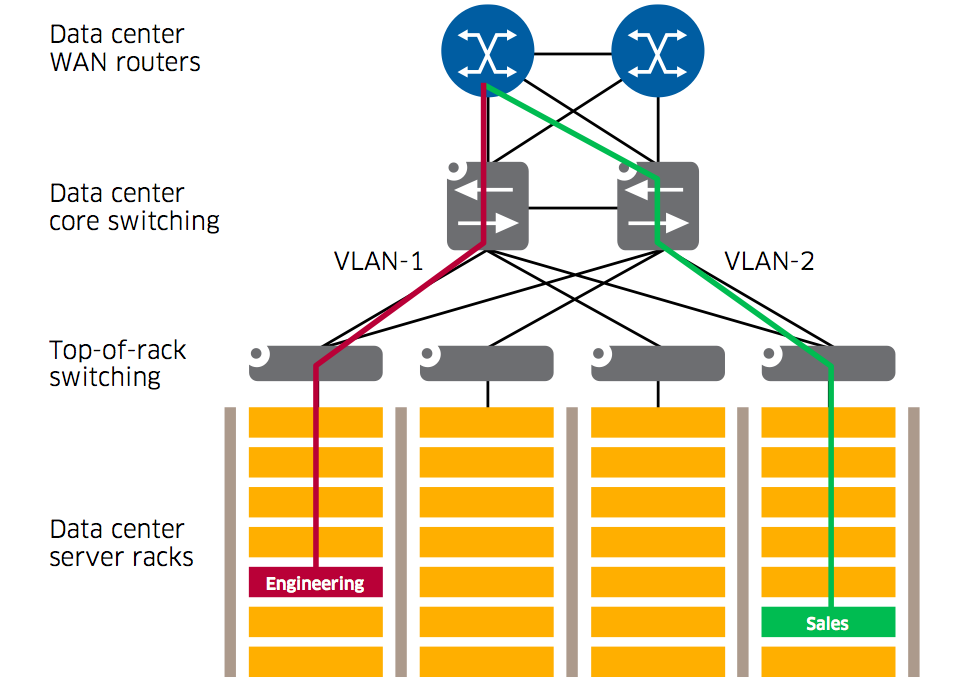
\includegraphics[width=0.6\textwidth]{images/AspecMultiTenant} 
\caption{Architecture réseau typique à trois niveaux. \cite{leveragingSDNCloudNetworkServiceExample}} \label{AspecMultiTenant}
\end{center}
\end{figure} 

Cette attribution doit être effectuée par le système de gestion des switches virtuels dans l'hyperviseur. Ensuite, la configuration doit être réalisée dans tous les switches du réseau data centre et dans le switch physique auquel le routeur est connecté. Quand le VLAN est déjà utilisé, l'interconnexion n'est pas possible, cela veut dire qu'une administration continue des VLANs attribués doit être mise en place. Tout cela est fait de manière fastidieuse et manuelle par l'opérateur du réseau.

Chaque réseau est connecté à un routeur, qui doit être configuré pour prendre en compte ces VLANs. Cela veut dire que le trafic doit toujours monter et descendre pour passer par ce router (réseau accès et de distribution), ce qui n'est pas très performant. La capacité du routeur peut limiter les communication inter-départements. 

Pour fournir des adresses IP automatiquement aux applications clients, un serveur DHCP doit être attribué à chaque réseau. L'équipe d'opération réseau met en place un serveur DHCP pour chaque réseau en accord avec les configurations dans les routeurs.

Le routeur doit implémenter les règles de sécurité pour permettre le trafic d'applications business entre les deux départements et l'accès internet. Les responsables de la sécurité doivent appliquer les politiques définies dans les interfaces du routeur pour assurer que seuls les flux de trafic permis sont transférés.

Cet exemple illustre la complexité opérationnelle de la configuration d'un réseau pour supporter une application. L'intervention exige un haut niveau de manipulation manuelle et concerne différents éléments de l'architecture. La totalité de la procédure est complexe et susceptible de provoquer diverses erreurs. Tout changement associé, comme le déplacement d'un serveur, l'extension d'un des réseaux, la modification de la configuration des tenants, implique quasiment la répétition complète du procédé et de la validation.

Dans le cas où la situation décrite doit être réalisée simultanément pour multiples consommateurs, il y aura clairement un grand délai d'implémentation. Dans un contexte Cloud, le traitement de demandes réseau durant plusieurs jours ou semaines devient critique et inacceptable.  \cite{hpCloudEffectsOnNetworkLimitations} \cite{leveragingSDNCloudNetworkServiceExample} \cite{zkCloudArrived}


\subsection{Interconnexion WAN}

Ce scénario illustre la connexion des réseaux tenants au WAN pour l'accès aux sites distants. Par exemple, on pourrait imaginer, dans le cas précédent, l'interconnexion des deux tenants proposés à un autre site de l'entreprise (image \ref{InterconnexionWAN}). Dans l'approche traditionnelle, un VLAN doit être créé entre le routeur du data centre et le routeur WAN.



\begin{figure}[h]
\begin{center}
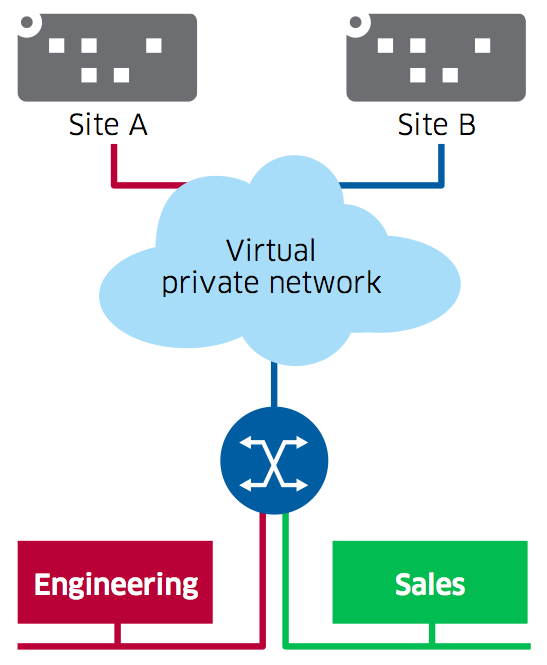
\includegraphics[width=0.4\textwidth]{images/InterconnexionWAN} 
\caption{Interconnexion des réseaux tenants sur deux sites. \cite{leveragingSDNCloudDCWAN}} \label{InterconnexionWAN}
\end{center}
\end{figure} 


%The example assumes a customer tenant configuration with two networks: one to be used by the engineering group, and the other by sales. The engineering department can only communicate with the sales department through web traffic; all other communication should be blocked. Both the engineering and sales teams are allowed to communicate with the Internet. 

Un protocole de routage doit être défini pour fournir une résilience en cas de failles de communication. La configuration doit être appliquée dans les deux routeurs impliqués. Pour offrir des mécanismes anti-failles aux niveaux 2 et 3 dans le WAN, plusieurs points VPNs doivent être déployés et configurés, ce qui ajoute de la complexité dans l'opération.

Traditionnellement,  les réseaux du data centre et du WAN sont gérés  par des responsables distincts. Cela implique la coordination entre les deux personnels réseaux, en général via une structure formelle de projet et procédures manuelles. Par ailleurs, avec les demandes de divers tenants, ce modèle introduit des délais ainsi que des problèmes d'extensibilités supplémentaires lorsqu'ils requièrent des VLANs ou protocoles de routage dédiés.

Avec l'ajout de sites et tenants, une variété de requis et configurations doivent être gérés et la complexité de déploiement de ce scénario devient critique. L'hétérogénéité des systèmes impliqués impose des défis difficiles à surmonter avec des délais de réalisation incompatibles. \cite{leveragingSDNCloudDCWAN} \cite{zkCloudIntelligentNetwork}


\subsection{Monitoring dans un data centre}

Historiquement, les systèmes de monitoring se sont appuyés sur une variété de protocoles et une série fragmentée d'outils. Ces outils incluent la supervision de la performance du réseau, des applications et des analyses de sécurité, telles que \gls{ids} et \gls{ips}. En complément à l'inspection des paquets, ces outils utilisent plusieurs meta protocoles pour fournir des données sur les réseaux, tels que SNMP, NetFlow et sFlow.
%Historically, monitoring systems have relied on a variety of protocols and a fragmented set of tools. Such tools include network performance monitoring, application performance monitoring, and security analysis tools, such as IDS/IPS. In addition to packet data, those tools use any of several meta protocols for providing data about networks, such as SNMP, NetFlow, and sFlow.

L'ajout de ces outils à l'opération du réseau est le premier pas vers une visibilité opérationnelle, permettant de détecter et solutionner les problèmes plus rapidement. La difficulté qui reste est d'alimenter ces outils avec la redirection du trafic vers leurs capteurs, pour qu'ils puissent superviser et gérer la quantité massive de données passantes d'une manière flexible et efficace. 
%Adding those tools to network operations is the first step towards operational visibility.  The problem that remains, however, is stitching these tools to the traffic so that they can monitor and manage in a flexible, cost-effective manner. Sifting through terabytes of data or even getting access to the data has posed challenges, increasing the time to resolution for many network problems. Getting traffic to these tools is the root of many barriers to more efficient network troubleshooting and problem resolution.

La localisation des pannes est considérablement simplifiée si les données des paquets sont filtrées et rendues disponibles aux administrateurs du réseau. Précédemment, les flux de données circulaient principalement en direction Nord/Sud, le placement de la capture ou redirection du trafic était donc évident : dans les points d'entrée/sortie du réseau. Toutefois, avec les tendances actuelles de flux plutôt Est/Ouest, de mobilité des hôtes et de demandes plus importantes pour la performance, la supervision est devenue plus difficile et couteuse dans les data centres modernes.
%Troubleshooting is dramatically simplified if filtered packet data is available to network administrators. In the past, when most data center traffic egressed the local site and headed “north” to an external network or came inbound, for example from the Internet, there was an obvious place to tap traffic or install a probe. Monitoring the ports where traffic enters and exits a DMZ or by duplicating traffic on a port used by a load balancer were obvious points to monitor. Traffic patterns shifted dramatically, from the north-south model, where security boundaries and load-balancers provided an obvious place to capture traffic, to an east-west model where the traffic never leaves the local network and instead is sent to hosts within the data center. In a modern data center, host mobility, performance, and east-west traffic make monitoring more difficult and expensive.

Les approches initiales pour la résolution de ces problèmes étaient l'agrégation du trafic drainé à des systèmes haute performance et envoyé aux outils de monitoring. Dispositifs comme les \glspl{npb} offrent des fonctionnalités additionnelles telles que manipulation ou enregistrement de la charge utile. 
%Initial approaches to solving these problems involved aggregating tapped traffic in high performance systems and then forwarding that traffic to monitoring tools. Devices, such as NPBs, often offer additional features, like payload manipulation or recording.

Le déploiement de ces outils pour chaque tranche réseau des tenants n'est pas efficace, particulièrement quand plusieurs instances d'outils sont requises pour le traitement d'un trafic excessivement important pour être supporté par une seule instance. En outre, l'ajout d'instances et outils exige des attentes répétitives pour la maintenance et implique diverses étapes pour le routage du trafic, connexion de systèmes de drainage et ensuite réversion à la configuration de routage initiale. Tout cela effectué manuellement par l'administrateur réseau. Une fois déployées, ces solutions fixent le trafic statiquement à un ensemble d'outils, ce qui peut conduire au cloisonnement des informations et difficultés à les partager entre tenants. \cite{bigSwitchTapModernDC}
% Deploying tools to every “silo” within the network is inefficient, especially when multiple instances of tools are required because traffic levels are too high for a single instance to handle. Further, adding aggregation systems and tools sometimes requires repeated waits on maintenance windows, which can delay deployment or require multiple steps because traffic must first be routed around the desired port, then the tap must be added, and then administrator must revert to original routing configuration. These approaches, once deployed, fix the traffic to a single toolset in a static fashion, which can lead to “port contention” and “stove-piping,” where information available to one team is hidden or difficult for another team to access.

%\section{Différents usages}




%\section{Agilité}


\section{Aspects de sécurité}

Comme développé précédemment, on exige de nos jours que les applications livrent immédiatement des informations et services spécifiques au contexte, à une latence réduite et à une haute performance. Parallèlement, le Cloud Computing et les applications orientées services introduisent des demandes plus strictes au niveau service. La mutualisation de ressources et les infrastructures multi-tenantes ont apporté de nouvelles préoccupations pour la sécurité qui n'existaient pas précédemment et qui ne sont donc pas traitées dans l'architecture traditionnelle. Cette section a pour but d'aborder quelques menaces et questions de sécurité introduites par la virtualisation et le Cloud Computing.

%We expect web applications to deliver integrated, context-specific information and services. And, we expect it right now—low-latency, high performance connections are critical. At the same time, cloud computing and service-oriented applications are introducing more stringent service-level and security demands.



%Some security risks unique to a virtualization infrastructure include communication blind spots, inter-VM attacks, and mixed trust level VMs. Instant-on gaps and resource contention are also important considerations. This section addresses each of these threats and issues.



%communication Blind Spots
\textbf{Points invisibles de la communication}

Les applications de sécurité réseaux traditionnelles ne voient pas la communication entre VMs au sein du même hyperviseur, à moins que toutes leurs communications ne soient routées à l'extérieur de la machine hôte vers l'application de sécurité et re-routées à l'intérieur. Cette manière de traiter la problématique introduit un ralentissement considérable du réseau. 
%In virtualized environments, traditional network security appliances are blind to the communication between VMs on the same host unless all communications are routed outside the host machine to this separate appliance. But this security configuration introduces significant time lags. 

Dans le Cloud Computing, le moyen de traiter ce problème est d'intégrer des modules de sécurité dans chaque VM pour qu'elles puissent s'auto-protéger. Cette solution oblige la re-configuration de tous les systèmes en cas de mise à jour des politiques de sécurité. Il manque dans l'architecture actuelle un contrôleur central qui pourrait diffuser les politiques dans tous les nœuds. 
%Une manière de traiter ces deux problèmes est de placer une VM dédiée à la sécurité dans l'hôte qui gère la communication entre plusieurs VMs. La VM dédiée à la sécurité est intégrée à l'hyperviseur pour
%One way to eliminate blind spots while reducing time lags is to place a dedicated scanning security VM on the host that coordinates communication between VMs. This solution works well in a virtualized environment. However, a dedicated security VM is not ideal for a cloud environment. The dedicated security VM integrates with the hypervisor to communicate with other guest VMs. In some cloud environments, such as in a multi-tenant public cloud, users do not have access to the hypervisor. In the cloud, protection is best provided as self-defending VMs. Protection is self contained on each VM and does not require communication outside of the VM to remain secure.

%inter-Vm attacks and hypervisor compromises
\textbf{Attaques entre VMs et exposition de l'hyperviseur}

Les serveurs virtualisés utilisent les mêmes systèmes d'exploitation et applications que les serveurs physiques. Les vulnérabilités retrouvées alors représentent donc des menaces pour les systèmes physiques ainsi que pour les environnements virtuels. De cette manière, quand un élément de l'environnement virtuel est compromis, l'ensemble du système est en position de risque dès lors qu'un système de sécurité conscient de la virtualisation n'est pas en place. 
%Virtualized servers use the same operating systems, enterprise applications, and web applications as physical servers. Hence, the ability of an attacker to remotely exploit vulnerabilities in these systems and applications is a significant threat to virtualized environments as well. And once an attacker compromises one element of a virtual environment, oather elements may also be compromised if virtualization-aware security is not implemented.

Dans ce scénario, un hacker peut attaquer un système invité, qui peut ensuite infecter d'autres VMs. Le risque augmente avec le nombre de VMs hébergées. Une protection capable de détecter des activités malveillantes au niveau des VMs doit être mise en place, indépendamment de la localisation des VMs dans l'environnement virtuel.
%In one scenario, an attacker can compromise one guest VM, which can then pass the infection to other guest VMs on the same host. Co-location of multiple VMs increases the attack surface and risk of VM-to-VM compromise. A firewall and an intrusion detection and prevention system need to be able to detect malicious activity at the VM level, regardless of the location of the VM within the virtualized environment.

Un autre mode d'attaque concerne l'hyperviseur qui devient une cible d'attaque en raison de son rôle et ses responsabilités. Certaines attaques vont essayer de traverser l'espace d'isolation des VMs pour compromettre l'hyperviseur. Sécuriser l'hyperviseur est donc indispensable, malgré la complexité de réalisation.
%Another attack mode involves the hypervisor, which is the software that enables multiple VMs to run within a single computer. While central to all virtualization methods, hypervisors bring both new capabilities and computing risks. A hypervisor can control all aspects of all VMs that run on the hardware, so it is a natural security target. Therefore, securing a hypervisor is vital, yet more complex than it seems.

%In an attack known as “hyperjacking,” malware that has penetrated one VM may attack the hypervisor. When a guest VM attempts this attack, it is often called a “guest VM escape” because the guest VM breaks out of, or escapes, its isolated environment and attacks the host hypervisor. Once compromised, a hypervisor can then attack other guest VMs on that host.

%VMs make requests to the hypervisor through several different methods, usually involving a specific application programming interface (API) call. An API is the interface created to manage VMs from the host machine. These APIs are prime targets for malicious code, so virtualization vendors attempt to ensure that APIs are secure and that VMs make only authentic (i.e. authenticated and authorized) requests. Because this is a critical path function, speed is a significant requirement in all hypervisors to ensure that overall performance is not impeded.
%When attackers targeted a zero-day vulnerability in a virtualization application called HyperVM made by LXLabs, as many as 100,000 web sites were destroyed [1]. In addition, certain virtualization vendors like Amazon Web Services have made their APIs public. These will undoubtedly become interesting targets for cybercriminals. Vendors that have not made their APIs public like vSphere, while not usually externally exposed, can also become potential targets for attacks within their perimeters. There is a risk that, owing to the rapid change in the API space and the current race to market, virtualization management systems will not be secure in the future.

%mixed trust level Vms
\textbf{VMs à niveaux de confiance mixtes}

Les VMs qui contiennent des données sensibles peuvent finir par résider dans le même hôte qu'une autre VM moins critique, ce qui entraine différents niveaux de confiance dans un groupement de VMs. Il serait possible de séparer les VMs selon leurs niveaux de sécurité, mais ce principe contredit l'intention de la virtulisation de faire une meilleure utilisation des ressources. Cette problématique implique un système de protection par VM, malgré la complexité déjà évoquée à synchroniser les politiques entre tous les systèmes.
%VMs with mission-critical data may reside on the same host as VMs with less critical data – resulting in mixed trust level VMs. Enterprises can attempt to segregate these different levels of secure information on separate host machines, but in some cases, this can defeat the purpose of a virtualized environment – to make the most efficient use of resources. Enterprises need to ensure that mission-critical information is protected while still realizing the benefits of virtualization. With self-defending VM security, VMs can remain safe even in mixed trust level environments, with protection such as intrusion detection and prevention, a firewall, integrity monitoring, log inspection, and antivirus capabilities.

%instant-on gaps
\textbf{Lacunes sur les instantanées}

La virtualisation et le Cloud Computing apportent des fonctionnalités telles que : approvisionnement, clonage, migration et désaffectation à la demande. Il en résulte que les VMs sont activées et inactivées à cycles rapides et il peut être difficile d'assurer une sécurité efficace de ces systèmes tout en les gardant à jour.
%Virtualized environments are not necessarily inherently less secure than their physical counterparts. However, in some cases, the practical uses of virtualization can introduce vulnerabilities, unless administrators are aware of these vulnerabilities and take steps to eliminate them. Instant-on gaps are an example of such a vulnerability.
%Beyond server consolidation, enterprises take advantage of the dynamic nature of VMs by quickly provisioning, cloning, migrating, and decommissioning VMs as needed, for test environments, scheduled maintenance, and disaster recovery, and to support task workers who need computational resources on-demand. As a result, when VMs are activated and inactivated in rapid cycles, rapidly and consistently provisioning security to those VMs and keeping them up-to-date can be challenging.

Après une période d'inactivité, l'écart des VMs par rapport à la base de sécurité peut être tellement important que la simple mise sous tension peut introduire des vulnérabilités considérables. Par ailleurs, même les VMs inactives peuvent être compromises. De cette manière, de nouvelles VMs peuvent être clonées à partir de templates avec une sécurité obsolète et être mises en ligne.
%After a period of time, dormant VMs can eventually deviate so far from the baseline security state that simply powering them on introduces significant security vulnerabilities. And even if VMs are dormant, attackers may still be able to access them. Also, new VMs may be cloned from VM templates with out-of-date security. Even when VMs are built from a template with virus protection and other security applications, the VMs need the security agent to have the latest security configurations and pattern file updates.

Quand ces VMs sont réactivées ou clonées, elles représentent une vulnérabilité instantanée à partir du moment où elles sont connectées au réseau. Une solution serait l'installation,  pour chaque hôte, d'une VM dédiée pour la mise à jour des applications de sécurité des autres VMs qui sont lancées, ce qui permettrait de profiter des bénéfices de la virtualisation en toute sécurité. 
%When dormant, reactivated, or cloned VMs have out-of-date security, attackers may be able to leverage an exploit for a longer period of time – the attack may have more longevity. Generally, if a guest VM is not online during the deployment or updating of antivirus software, it will lie dormant in an unprotected state and be instantly vulnerable when it does come online. One solution is a dedicated security VM on each host that automatically updates VMs with the latest security when activated or cloned, and safely allows enterprises to realize the benefits of virtualization.

%resource contention 
\textbf{Blocage de ressources}

Quand des opérations gourmandes en ressources sont appliquées aux VMs, elle peuvent rapidement surcharger le système. Par exemple, quand les balayages ou mise-à-jour des antivirus sont réalisés simultanément sur plusieurs VMs dans un même serveur physique, le système peut ne pas supporter la consommation intensive des ressources (mémoire, CPU, réseau, stockage). Cela peut impacter la performance globale des applications en exécution.
%When resource intensive operations such as regular antivirus scans and pattern file updates designed for physical environments are applied to VMs, these operations can quickly result in an extreme load on the system. When antivirus scans or scheduled updates simultaneously kick into action on all VMs on a single physical system, the result is an antivirus storm. This storm is like a run on the bank, where the bank is the underlying virtualized resource pool of memory, storage, and CPU. This performance impact hampers server applications and VDI environments.

Dans les systèmes physiques, des anti-virus installés dans chaque système d'exploitation consomment une mémoire additionnelle importante. L'application de cette architecture aux systèmes virtuels signifie une perte indésirable d'efficacité sur l'utilisation des ressources. Les produits qui ignorent la virtualisation proposent la randomisation ou le regroupement pour éviter la charge intensive d'opérations simultanées.
%The legacy security architecture also results in linear growth of memory allocation as the number of VMs on a single host grows. In physical environments, antivirus software must be installed on each operating system. Applying this architecture to virtual systems means that each VM requires additional significant memory footprint  an unwanted drain on server consolidation efforts. Products that are not virtualization-aware suggest the use of randomization or grouping to avoid resource contention.

Malheureusement, la randomisation ne permet pas d'éviter les longues périodes de haute consommation du système pour les cycles complets de balayage. Le groupement ne contribue pas à la nature mobile de la virtualisation et exige une reconfiguration lors de la migration ou du clonage de VMs. 
%"Grouping does not allow for the mobile nature of virtualization, requiring reconfiguration when VMs are migrated or cloned."
%However, randomization does not help to avoid times of high system usage and requires that a long period of time be reserved for the full scan cycle. Grouping does not allow for the mobile nature of virtualization, requiring reconfiguration when VMs are migrated or cloned.

\cite{cloudSecurityThreats}


\section{Complexité, Agilité et Sécurité : l'adaptation du réseau au Cloud}

Les applications data centres ont évolué vers un modèle beaucoup plus dynamique pour accompagner le rythme des demandes des consommateurs Cloud Computing. Ce nouveau mode de livraison et consommation exige une infrastructure beaucoup plus flexible, capable de s'adapter rapidement pour fournir les ressources sollicitées. 

En vue des scénarios étudiés, l'agilité est devenue cruciale dans ce contexte où les décisions se font de plus en plus en temps réel. Cet objectif ne peut pas être atteint sans la mise en place d'outils pour automatiser et orchestrer les éléments dans l'infrastructure. Dans l'aspect réseau, diverses opérations nécessaires sont toujours essentiellement manuelles et freinent le passage à ce modèle.

Le nombre de modules à gérer et ses interfaces implique des contraintes pour le déploiement de nouvelles applications et services. La réponse aux divers cas d'utilisation Cloud Computing impose à la fois des opérations manuelles et une complexité de réalisation. Le développement d'outils pour automatiser ces scénarios introduit encore plus de complexité et ne s'adapte pas à tout data centre selon les modèles des équipements et protocoles utilisés.

En plus de ces exigences difficiles à traiter au moyen des réseaux traditionnels, l'environnement Cloud Computing exige une sécurité plus élevée du \gls{si}. Dans ce modèle, la performance, la haute disponibilité et la protection de données sont requises à un niveau plus important par rapport aux data centres traditionnels. L'architecture réseau actuelle n'est pas adaptée aux questions de sécurité ressortant de la virtualisation et du Cloud.

En résumé, il est difficile aujourd'hui d'atteindre le niveau d'agilité et sécurité exigé avec les technologies réseaux classiques sans introduire une complexité excessivement contraignante et donc bloquante pour la libération du Cloud Computing. Dans le chapitre suivant, il sera analysé de nouvelles applications SDN qui proposent des solutions pour aborder ces problématiques. 